%!TEX program = lualatex -shell-escape
\documentclass[
    hyperref={colorlinks,linkcolor=blue,urlcolor=blue,citecolor=blue}
]{beamer}
\mode<presentation> {
    \usetheme{metropolis}
}
\usepackage[polish]{babel}
\usepackage[autostyle=true]{csquotes}
\usepackage{fontspec}
\usepackage{amsmath}
\usepackage{mathtools}
\usepackage{xcolor}
\usepackage{fdsymbol}
\usepackage{enumitem}
\usepackage{array}
\usepackage{csquotes}
\usepackage{fontawesome5}
\usepackage{animate}
\usepackage{tcolorbox}
% Biber configuration
\usepackage[
    backend=biber,
    style=alphabetic,
    citestyle=authoryear,
    natbib
]{biblatex}
% TikZ configuration
\usepackage{tikz}
\usepackage{pgfplots}
\usetikzlibrary{
    shapes,
    shapes.geometric,
    positioning,
    shadows,
    trees,
    calc,
    arrows,
    fit
}
\tikzset{
  basic/.style = {
      draw,
      text width=1.5cm,
      drop shadow,
      font=\sffamily,
      rectangle,
      fill=lightgray!30,
      align=center
  },
  round/.style = {
    basic,
    rounded corners=2pt,
    thin
  },
  rhombus/.style = {
    basic,
    diamond
  },
  simple/.style = {
      basic,
      thin,
      text width=3em
  },
  plain/.style = {
      draw=none
  },
  label/.style = {
      font=\large\bfseries
  },
  main node/.style = {
      circle,
      fill=blue!20,
      draw,
      minimum size=1cm,
      inner sep=0pt
  },
  vertex/.style = {
      draw,
      circle,
      drop shadow,
      font=\sffamily,
      align=center,
      color=white,
      fill=black
  },
  edge/.style = {
      ultra thick
  },
  weight/.style = {
    label,
    circle,
    fill=white,
    draw,
    minimum size=3mm,
    inner sep=1pt
  },
  ego/.style = {
      vertex,
      color=white,
      fill=red
  }
}

% Configure section slides insertion
\AtBeginSection[]{
  \begin{frame}
  \vfill
  \centering
  \begin{beamercolorbox}[sep=8pt,center,shadow=true,rounded=true]{title}
    \usebeamerfont{title}\insertsection\par%
  \end{beamercolorbox}
  \vfill
  \end{frame}
}

% Bibliography and graphics paths
\addbibresource{literature.bib}
\graphicspath{{./../../figures/}}

% Beamer settings
% \setbeamercovered{transparent}
\setbeamercovered{invisible}
\setbeamercovered{%
  again covered={\opaqueness<1->{15}}}

% Unnumbered footnotes
\newcommand\blfootnote[1]{%
    \let\thefootnote\relax\footnotetext{#1}
}

% Place logo in the footer
\setbeamertemplate{footline}{%
    \hypersetup{urlcolor=black!10}
    % \hspace{1em}
    \begin{minipage}{.2\textwidth}
        \setbeamercolor*{logobg}{fg=black!80, bg=white}
        \begin{beamercolorbox}{logobg}
            \hspace{1em}
            
\includegraphics[height=.75cm]{UW-logo.png}%
        \end{beamercolorbox}
        \vspace{1em}
    \end{minipage}
    \hfill%
    \begin{minipage}{.79\textwidth}
    % \begin{minipage}{.45\textwidth}
    %     \hfill
    %     \setbeamercolor*{twitter}{fg=black!10, bg=black!50}
    %     \begin{beamercolorbox}[wd=12em, ht=1.8em]{twitter}%
    %         \hspace{.5em}
    %         \begin{minipage}{2em}
    %         \scriptsize{%
    %             \faIcon{twitter}
    %         }
    %         \vspace{.1em}
    %         \end{minipage}
    %         % \textbf{\scriptsize{
    %         %     \texttt{\href{https://twitter.com/\_stalaga\_}{@\_stalaga\_}}%
    %         % }}
    %         \vspace{.15em}
    %     \end{beamercolorbox}%
    %     \vspace{.4em}
    % \end{minipage}
    % \hspace{-.7em}
    \hfill
    \begin{minipage}{.75\textwidth}
        \setbeamercolor*{footline}{fg=white, bg=black!80}
        \centering
        \begin{beamercolorbox}[ht=1.8em]{footline}%
            \hspace{1em}
            \centering{\scriptsize{%}
                \textbf{Sociology of Elites: Case Studies and methods}
            }}
            \vspace{.2em}
        \end{beamercolorbox}%
        \vspace{.4em}
    \end{minipage}
    \vspace{.6em}
    \end{minipage}
    \vspace{-1em}
}

% Math symbols
\newcommand{\N}{\ensuremath{\mathbb{N}}}
\newcommand{\Z}{\ensuremath{\mathbb{Z}}}
\newcommand{\R}{\ensuremath{\mathbb{R}}}
\newcommand{\Prob}{\ensuremath{\mathbb{P}}}
\newcommand{\E}{\ensuremath{\mathbb{E}}}

\newcommand{\indep}{\raisebox{0.05em}{\rotatebox[origin=c]{90}{$\models$}}}

% Math font styling
\mathversion{bold}
\everydisplay{\color{black}}

% Colors
\newcommand{\green}[1]{\textcolor{black!40!green}{#1}}
\newcommand{\red}[1]{\textcolor{red}{#1}}
\newcommand{\yellow}[1]{\textcolor{black!10!red!30!yellow}{#1}}
\newcommand{\blue}[1]{\textcolor{white!30!blue}{#1}}
\newcommand{\gray}[1]{\textcolor{black!20}{#1}}

% Custom sets

% Fix enumerate environment
\def\labelenumi{\theenumi.}

% Use white background for slides
\setbeamercolor{background canvas}{bg=white}

%%%%%%%%%%%%%%%%%%%%%%%%%%%%%%%%%%%%%%%%%%%%%%%%%%%%%%%%%%%%%%%%%%%%%%%%%%%%%%%
\begin{document}

% Title and authors
\title[Structure of networks]{
    Introduction to Network Science:\\structure of networks
}
\author{Szymon Talaga$^1$}
\institute[ISS UW]{
    $^1$ Robert Zajonc Institute for Social Studies,
    University of Warsaw \\
    \medskip

    \faIcon{envelope}\enspace
    \textcolor{blue}{\href{mailto:stalaga@uw.edu.pl}{stalaga@uw.edu.pl}} \\
    \faIcon{address-card}
    \href{http://iss.uw.edu.pl/en/szymon-talaga/}{iss.uw.edu.pl/en/szymon-talaga}
}
\date{
    October 15, 2021 \\
} % Date, can be changed to a custom date

%%% SLIDES %%%%%%%%%%%%%%%%%%%%%%%%%%%%%%%%%%%%%%%%%%%%%%%%%%%%%%%%%%%%%%%%%%%%
\frame{\titlepage}

\section{Introduction}

\begin{frame}{Opening remarks}
\begin{itemize}
    \item<2-> Time is short, so we will only scratch the surface.
    \item<3-> We will skip technical/mathematical details as much as possible.
    \item<4-> Instead, the focus will be on conceptual understanding and
    practical computing.
\end{itemize}
\end{frame}

\section{Clustering \& network communities}

\begin{frame}{My friends are friends with each other \ldots}
\begin{itemize}
    \item<1-> It is quite common that our friends know each other and that
    we are friends with our friends.
    \item<2-> This is a process known in sociology as triadic closure.
    \item<3-> And since this is about relations between different individuals
    or entities, then it is natural to ask, what is the network view of this?
\end{itemize}
\end{frame}

\begin{frame}{Local clustering coefficient \& triadic closure}
\begin{center}
\begin{tikzpicture}[node distance=1.5cm]
    % Nodes
    \node[ego] (n1) {$1$};
    \node[vertex, below left of=n1] (n2) {$2$};
    \node[vertex, below right of=n1] (n3) {$3$};
    % Edges
    \path[draw, ultra thick]
    (n1) edge (n2)
    (n1) edge (n3);
    \pause
    \path[draw, ultra thick, dotted]
    (n2) -- (n3);
    \pause
    \path[draw, ultra thick]
    (n2) -- (n3);
\end{tikzpicture}
\end{center}
\pause
\begin{itemize}
    \item<4-> Local clustering coefficient of a node $i$ is defined as:
    \[
        c_i =
        \frac{\text{\# number of triangles including \ensuremath{i}}}{%
        \text{\# of triples with \ensuremath{i} in the middle}%
    }
    \]
    \item<5-> It measures the extent to which:
    \begin{quote}
        My friends are friends with each other
    \end{quote}
\end{itemize}
\end{frame}

\begin{frame}{Local clustering coefficient | Some remarks}
\begin{itemize}
    \item<2-> It does not capture the extent to which:
    \begin{quote}
        Friends of my friends are my friends
    \end{quote}
\end{itemize}
\pause
\pause
\begin{center}
\begin{tikzpicture}[node distance=1.5cm]
    % Nodes
    \node[ego] (n1) {$1$};
    \node[vertex, below left of=n1] (n2) {$2$};
    \node[vertex, below right of=n1] (n3) {$3$};
    \node[vertex, below left of=n2] (n4) {$4$};
    \node[vertex, below right of=n2] (n5) {$5$};
    \node[vertex, below right of=n3] (n6) {$6$};
    % Edges
    \path[draw, ultra thick]
    (n1) edge (n2)
    (n1) edge (n3)
    (n2) edge (n3)
    (n4) edge (n2)
    (n5) edge (n2)
    (n6) edge (n3);
\end{tikzpicture}
\end{center}
\pause
\begin{itemize}
    \item Node $1$ clearly has maximum local clustering since both of its
    neighbors are connected. However, it is not connected
    to any neighbors of its own neighbors, which means that it does
    not \enquote{know friends of its friends}.
\end{itemize}
\end{frame}

\begin{frame}{Local clustering coefficients | Some remarks}
\begin{itemize}
    \item<2-> There are some alternative solutions addressing this problem.
    \item<3-> However, there are not very widely used yet, so due to time
    constraints we will not discuss them.
\end{itemize}
\end{frame}

\begin{frame}{Global clustering}
\begin{itemize}
    \item<2-> It is very often of interest to calculate some global measure
    of clustering for an entire network.
    \item<3-> One solution is to just calculate average local clustering.
    \item<4-> But this is problematic as local clustering is not defined
    for nodes of degree $1$ (do you see why?)
\end{itemize}
\end{frame}

\begin{frame}{Undefined local clustering coefficient}
\begin{center}
\begin{tikzpicture}[node distance=1.5cm]
    % Nodes
    \node[ego] (n1) {$1$};
    \node[vertex, below left of=n1] (n2) {$2$};
    \node[vertex, below right of=n2] (n3) {$3$};
    \node[vertex, below left of=n2] (n4) {$4$};
    % Edges
    \path[draw, ultra thick]
    (n1) edge (n2)
    (n2) edge (n3)
    (n2) edge (n4)
    (n3) edge (n5);
\end{tikzpicture}
\end{center}
\pause
\begin{itemize}
    \item There is no triple with $1$ in the middle.
\end{itemize}
\end{frame}

\begin{frame}{Global clustering coefficient}
\begin{itemize}
    \item<2-> This is why it is often better to calculate global
    clustering coefficient.
    \item<3-> It is defined as:
    \[
        \frac{%
            3 \times \text{\# of triangles}
        }{%
            \text{\# of triples}
        }
    \]
\end{itemize}
\end{frame}

\begin{frame}{Meaning of clustering}
\begin{itemize}
    \item<2-> Despite their imperfections, clustering coefficients are indicative
    of a very important structural property.
    \item<3-> They tell us something, even if usually not everything,
    about \textbf{how dense are local connections between different nodes}.
    \item<4-> This is important as densely connected regions within networks
    often correspond to \textbf{functionally distinct and significant parts
    of the system}.
\end{itemize}
\end{frame}

\begin{frame}{Expected clustering under ER model}
\begin{itemize}
    \item What is the expected clustering coefficient in the ER model?
\end{itemize}
\pause
\begin{center}
\begin{tikzpicture}[node distance=1.5cm]
    % Nodes
    \node[ego] (n1) {$1$};
    \node[vertex, below left of=n1] (n2) {$2$};
    \node[vertex, below right of=n1] (n3) {$3$};
    % Edges
    \path[draw, ultra thick]
    (n1) edge (n2)
    (n1) edge (n3);
    \pause
    \path[draw, ultra thick, dotted]
    (n2) -- (n3);
    \pause
    \path[draw, ultra thick]
    (n2) -- (n3);
\end{tikzpicture}
\end{center}
\pause
\begin{itemize}
    \item It is simply $p$ as any edge in an ER random graph exists (or not)
    independently from other edges with probability $p$.
\end{itemize}
\end{frame}

\begin{frame}{Network communities}
\begin{itemize}
    \item<2-> The problem of finding dense subgraphs is studied in much more
    detailed within the framework of \textbf{community detection}.
    \item<3-> Community detection methods are algorithmic heuristics and/or
    principled statistical tools used to find dense subgraphs, which may
    correspond as functionally semi-separate entities.
    \item<4-> There is a whole zoo of community detection method, but here
    we will discuss only one of the most famous (and effective) algorithms.
\end{itemize}
\end{frame}

\begin{frame}{Network communities | Remark on structure}
\begin{itemize}
    \item<1-> For the sake of simplicity we will assume that communities
    correspond to subgraphs which has significantly higher edge densities
    than their surroundings.
    \item<2-> But the notion of communities is much more general than that
    and refers to many different kinds of characteristic network substructures.
    \item<3-> As a matter of fact, the algorithm we will discuss can detect
    communities of many different shapes.
\end{itemize}
\end{frame}

\begin{frame}{Shortest paths \& betwenness centrality}
\begin{itemize}
    \item<1-> Before we can discuss our community detection algorithm of choice
    we first have to introduce some additional basic notions.
    \item<2-> Shortest path between two nodes $i$ and $j$ is, well,
    the shortest possible path between them (there may be multiple equally
    short paths).
    \item<3-> We will later use the notion of shortest paths to define a new
    centrality measure known as \textbf{betweenness}, which is central
    for the community detection algorithm we want discuss.
\end{itemize}
\end{frame}

\begin{frame}{Shortest path | Example}
\begin{center}
\begin{tikzpicture}[node distance=1.5cm]
    % Nodes
    \node[ego] (n1) {$1$};
    \node[vertex, above right of=n1] (n2) {$2$};
    \node[vertex, below right of=n1] (n3) {$3$};
    \node[ego, above right of=n3] (n4) {$4$};
    \node[vertex, right of=n3] (n5) {$5$};
    % Edges
    \path[draw, ultra thick]
    (n1) edge (n2)
    (n1) edge (n3)
    (n2) edge (n4)
    (n3) edge (n4)
    (n3) edge (n5)
    (n5) edge (n4);
\end{tikzpicture}
\end{center}
\begin{itemize}
    \item<2-> $1-2-4$ is a shortest path between $1$ and $4$ (has length $2$).
    \item<3-> $1-3-4$ is a shortest path between $1$ and $4$ (has length $2$).
    \item<4-> $1-3-5-4$ \textbf{is not} a shortest path (has length $3$).
\end{itemize}
\end{frame}

\begin{frame}{Betweenness}
\begin{itemize}
    \item<2-> Betweenness of a node $i$ is the number of shortest paths
    between any two nodes in the network that go through it.
    \item<3-> \[
        b_i = \sum_{k, l \neq = i} \left(\text{%
            \# of shortest paths from \ensuremath{k} to \ensuremath{l}
            which go through \ensuremath{i}
        }\right)
    \]
    \item<4-> Unlike node degree it is a global measure of centrality
    which takes into account the whole structure of the network.
    \item<5-> By definition it is only loosely constrained by degree.
\end{itemize}
\end{frame}

\begin{frame}{Node with degree $1$ cannot have high betweenness \ldots}
\begin{center}
\begin{tikzpicture}[node distance=1.5cm]
    % Nodes
    \node[ego] (n1) {$1$};
    \node[vertex, below of=n1] (n2) {$2$};
    \node[vertex, below left of=n2] (n3) {$3$};
    \node[vertex, below right of=n2] (n4) {$4$};
    % Edges
    \path[draw, ultra thick]
    (n1) -- (n2)
    (n2) -- (n3)
    (n2) -- (n4)
    (n3) -- (n4);
\end{tikzpicture}
\end{center}
\end{frame}

\begin{frame}{\ldots{ }but a node with degree at least $2$ can}
\begin{center}
\begin{tikzpicture}[node distance=1.5cm]
    % Nodes
    \node[ego] (n1) {$1$};
    \node[vertex, above of=n1] (n2) {$2$};
    \node[vertex, above left of=n2] (n3) {$3$};
    \node[vertex, above right of=n2] (n4) {$4$};
    \node[vertex, below of=n1] (n5) {$5$};
    \node[vertex, below left of=n5] (n6) {$6$};
    \node[vertex, below right of=n5] (n7) {$7$};
    % Edges
    \path[draw, ultra thick]
    (n1) -- (n2) -- (n3) -- (n4)
    (n1) -- (n5) -- (n6) -- (n7)
    (n2) -- (n4)
    (n5) -- (n7);
\end{tikzpicture}
\end{center}
\end{frame}

\begin{frame}{Edge betweenness}
\begin{itemize}
    \item<1-> A convenient feature of betweenness centrality is that
    it can be defined also for edges.
    \item<2-> The definition in this case is exactly analogous.
    \item<3-> Edge betweenness measures the amount of shortest paths
    that travels through a particular edge.
\end{itemize}
\end{frame}

\begin{frame}{Modularity}
\begin{itemize}
    \item<1-> One last bit of network knowledge we need is the notion of
    \textbf{modularity}.
    \item<2-> Modularity is a function of a networks (its structure) and
    a particular partition of the nodes into non-overlapping groups.
    \item<3-> It is a normalized quantity which measures the extent to which
    edges within groups are denser than between groups.
\end{itemize}
\end{frame}

\begin{frame}{Girvan-Newman algorithm}
\begin{itemize}
    \item<2-> It is arguably one of the most famous and still widely used
    community detection algorithms.
    \item<3-> It is quite general and very effective for many types of networks.
    \item<4-> However, it is not super efficient in terms of computation time
    and may run relatively slowly for large networks.
    \pause
    \vspace{1em}
    \begin{columns}
    \column{.5\textwidth}
        \centering
        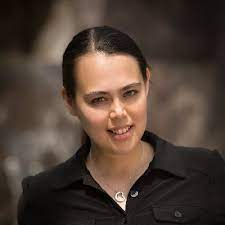
\includegraphics[width=.6\textwidth]{girvan}
    \column{.5\textwidth}
        \centering
        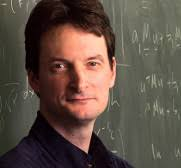
\includegraphics[width=.65\textwidth]{newman}
    \end{columns}
\end{itemize}
\end{frame}

\begin{frame}{Girvan-Newman algorithm | Heuristic}
\begin{itemize}
    \item<2-> Edges with high betweenness are exactly those that are instrumental
    for connecting different, otherwise sparsely connected, components.
    \item<3-> So if we start deleting edges with highest betweenness one-by-one
    we will systematically decompose the network into meaningful components.
\end{itemize}
\end{frame}

\begin{frame}{Girvan-Newman algorithm | Outline of the main loop}
\begin{enumerate}
    \item Find the edge with maximum betweenness.
    \item Remove it.
    \item Decompose the network into components. Separate components give
    the split into communities.
    \item Recalculate edge betweenness (that is the computationally hard part).
    \item Repeat from (1) until each node is in its own component
    (there are no edges left).
    \item Choose the split which maximizes the modularity score for the
    best solution.
\end{enumerate}
\end{frame}

\begin{frame}{Girvan-Newman algorithm | Example}
\begin{center}
    \begin{tikzpicture}[node distance=1.5cm]
        % Nodes
        \node[vertex] (n1) {$1$};
        \node[vertex, above of=n1] (n2) {$2$};
        \node[vertex, above left of=n2] (n3) {$3$};
        \node[vertex, above right of=n2] (n4) {$4$};
        \node[vertex, below of=n1] (n5) {$5$};
        \node[vertex, below left of=n5] (n6) {$6$};
        \node[vertex, below right of=n5] (n7) {$7$};
        % Edges
        \path[draw, ultra thick]
        (n1) -- (n2) -- (n3) -- (n4)
        (n1) -- (n5) -- (n6) -- (n7)
        (n2) -- (n4)
        (n5) -- (n7);
        \pause
        \draw[edge, color=red] (n1) -- (n2);
    \end{tikzpicture}
    \end{center}
\end{frame}

\begin{frame}{Girvan-Newman algorithm | Example}
\begin{center}
\begin{tikzpicture}[node distance=1.5cm]
    % Nodes
    \node[vertex] (n1) {$1$};
    \node[vertex, above of=n1] (n2) {$2$};
    \node[vertex, above left of=n2] (n3) {$3$};
    \node[vertex, above right of=n2] (n4) {$4$};
    \node[vertex, below of=n1] (n5) {$5$};
    \node[vertex, below left of=n5] (n6) {$6$};
    \node[vertex, below right of=n5] (n7) {$7$};
    % Edges
    \path[draw, ultra thick]
    (n2) -- (n3) -- (n4)
    (n1) -- (n5) -- (n6) -- (n7)
    (n2) -- (n4)
    (n5) -- (n7);
\end{tikzpicture}
\end{center}
\end{frame}

\begin{frame}{Girvan-Newman algorithm | Example}
\begin{center}
\begin{tikzpicture}[node distance=1.5cm]
    % Nodes
    \node[vertex] (n1) {$1$};
    \node[ego, above of=n1] (n2) {$2$};
    \node[ego, above left of=n2] (n3) {$3$};
    \node[ego, above right of=n2] (n4) {$4$};
    \node[vertex, below of=n1] (n5) {$5$};
    \node[vertex, below left of=n5] (n6) {$6$};
    \node[vertex, below right of=n5] (n7) {$7$};
    % Edges
    \path[draw, ultra thick]
    (n2) -- (n3) -- (n4)
    (n1) -- (n5) -- (n6) -- (n7)
    (n2) -- (n4)
    (n5) -- (n7);
\end{tikzpicture}
\end{center}
\end{frame}

\section{Small worlds}

\begin{frame}{Small world experiment}
\begin{itemize}
    \item<1-> In 1960's Jeffrey Travers and Stanley Milgram sent letters
    to $296$ random persons asking them to pass the letter to a specific
    person in a different state. Crucially they were allowed to pass the
    letter through intermediaries if they could not reach the target person
    directly.
    \item<2-> $217$ persons passed the letter further and $64$ messages
    (about $29.4\%$) eventually reached the target person.
    \item<3-> The average number of persons along a chain from a starting
    person to the target person was $5.2$.
\end{itemize}
\end{frame}

\begin{frame}{Small world experiment}
\centering
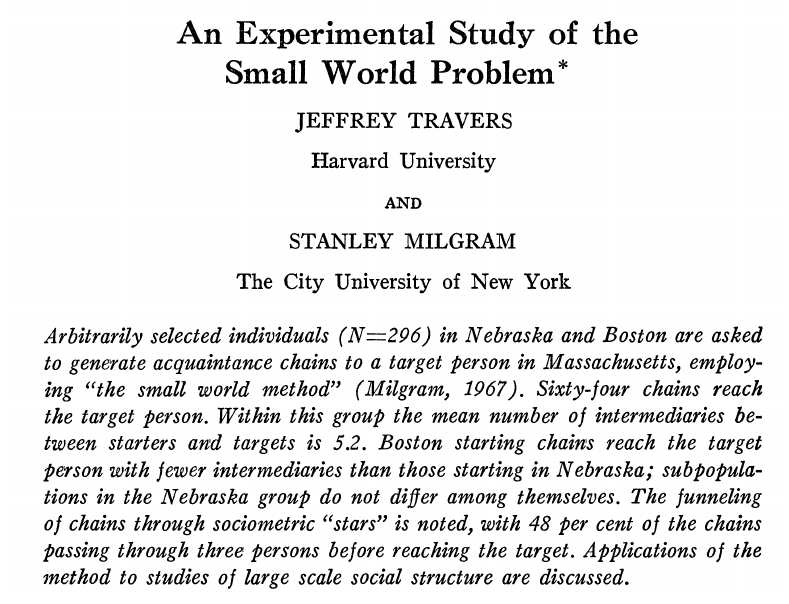
\includegraphics[width=.9\textwidth]{small-world-experiment.png}
\end{frame}

\begin{frame}{Replications of the experiment}
\begin{itemize}
    \item The experiment was replicated many times and in different context
    including very large online systems.
    \item<2-> In each and every case the average path length was very small,
    ranging roughly from $4$ to a dozen.
    \item<3-> So it seems that real networks have some structural
    properties that make shortest paths between arbitrary nodes very
    short on average irrespective of the size of the system.
\end{itemize}
\end{frame}

\begin{frame}{Average shortest paths in ER model}
\begin{itemize}
    \item<2-> On one hand this is not surprising as one of the early results
    of network science established that average shortest path length($L$) in
    ER model is proportional to the logarithm of the number of nodes:
    \[
        L \propto \log{N}
    \]
    \item<3-> But real networks are not much like the ER random graphs.
    \item<4-> So the question is, how is this possible even in networks
    with non trivial structure such as high clustering.
\end{itemize}
\end{frame}

\begin{frame}{Small-world model of Watts \& Strogatz}
\begin{itemize}
    \item In 1998 Watts and Strogatz came up with a very simple model
    exhibiting almost arbitrary large clustering and short average paths
    comparable to those in the ER model.
\end{itemize}
\end{frame}

\begin{frame}{Small-world model}
\centering
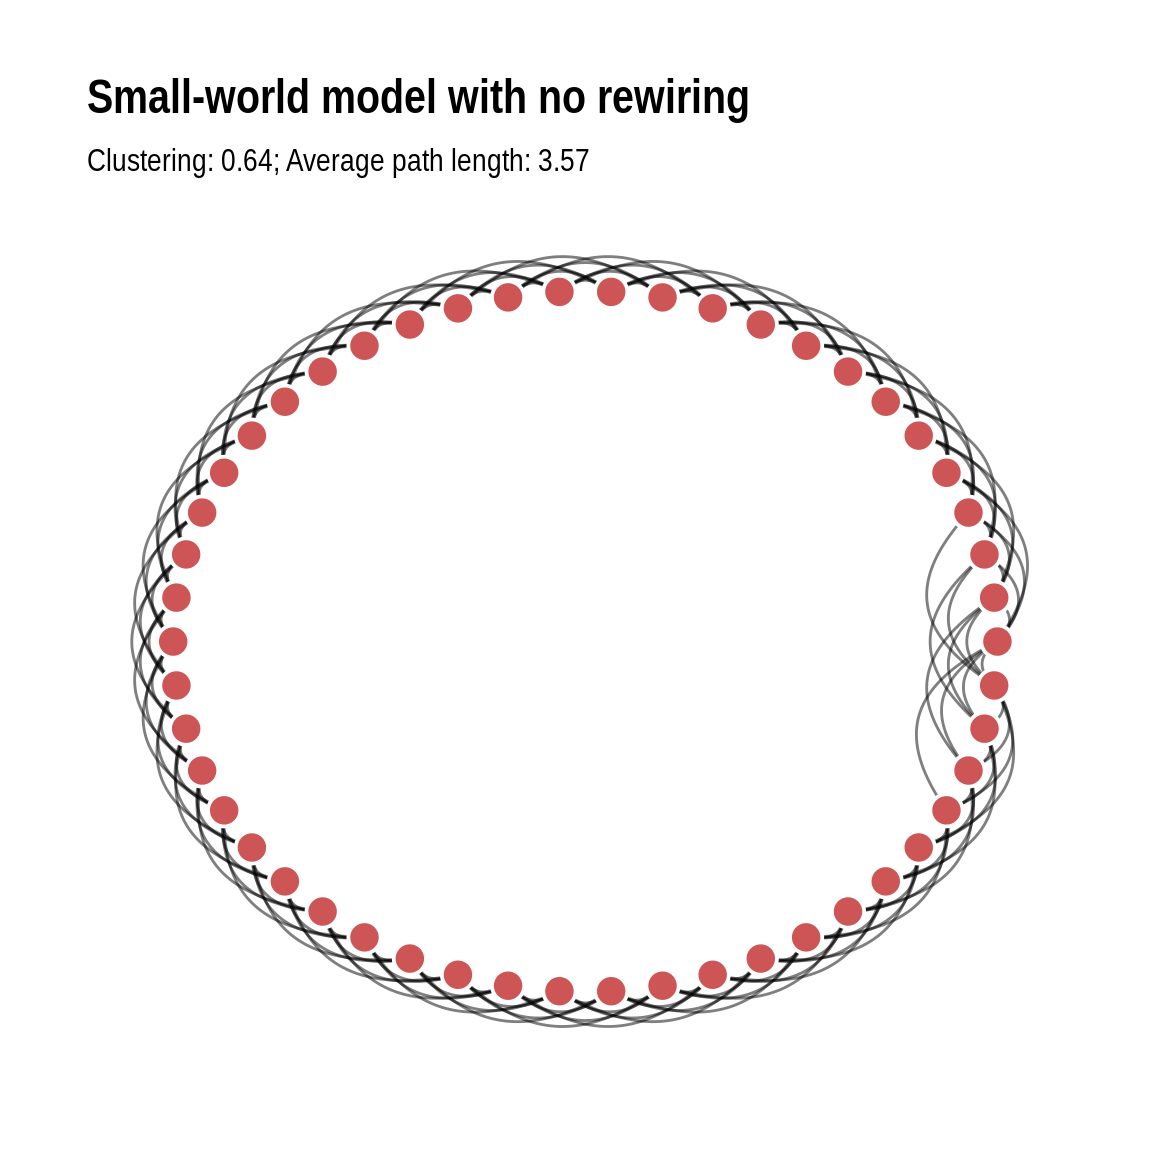
\includegraphics[width=.7\textwidth]{structure/small_world_no_rewiring-1}
\end{frame}

\begin{frame}{Small-world model}
\centering
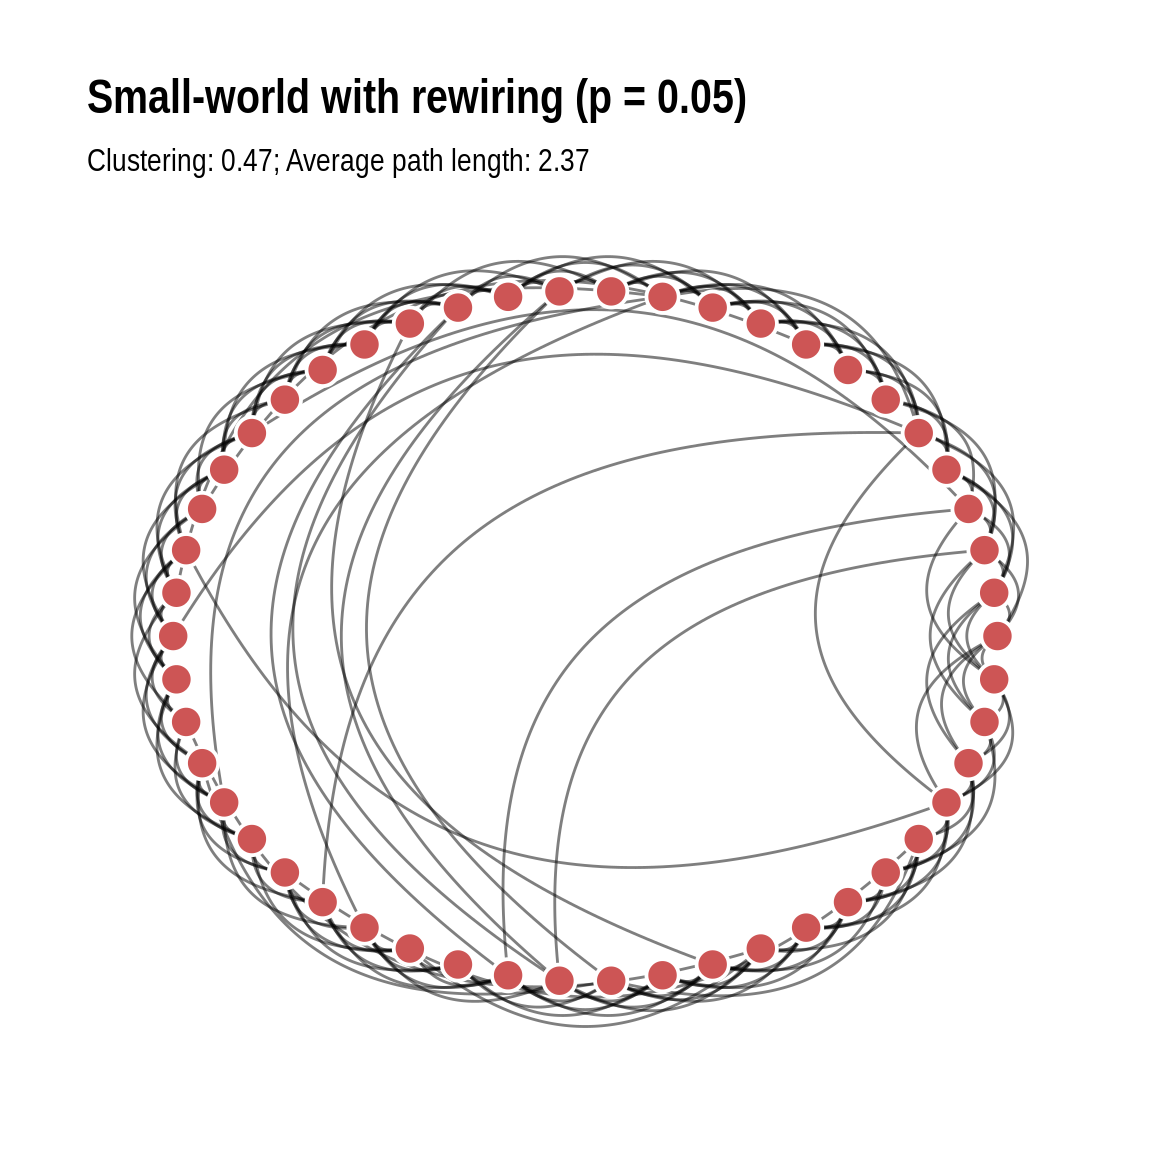
\includegraphics[width=.7\textwidth]{structure/small_world_with_rewiring-1}
\end{frame}

\begin{frame}{Small-world model | General result}
\centering
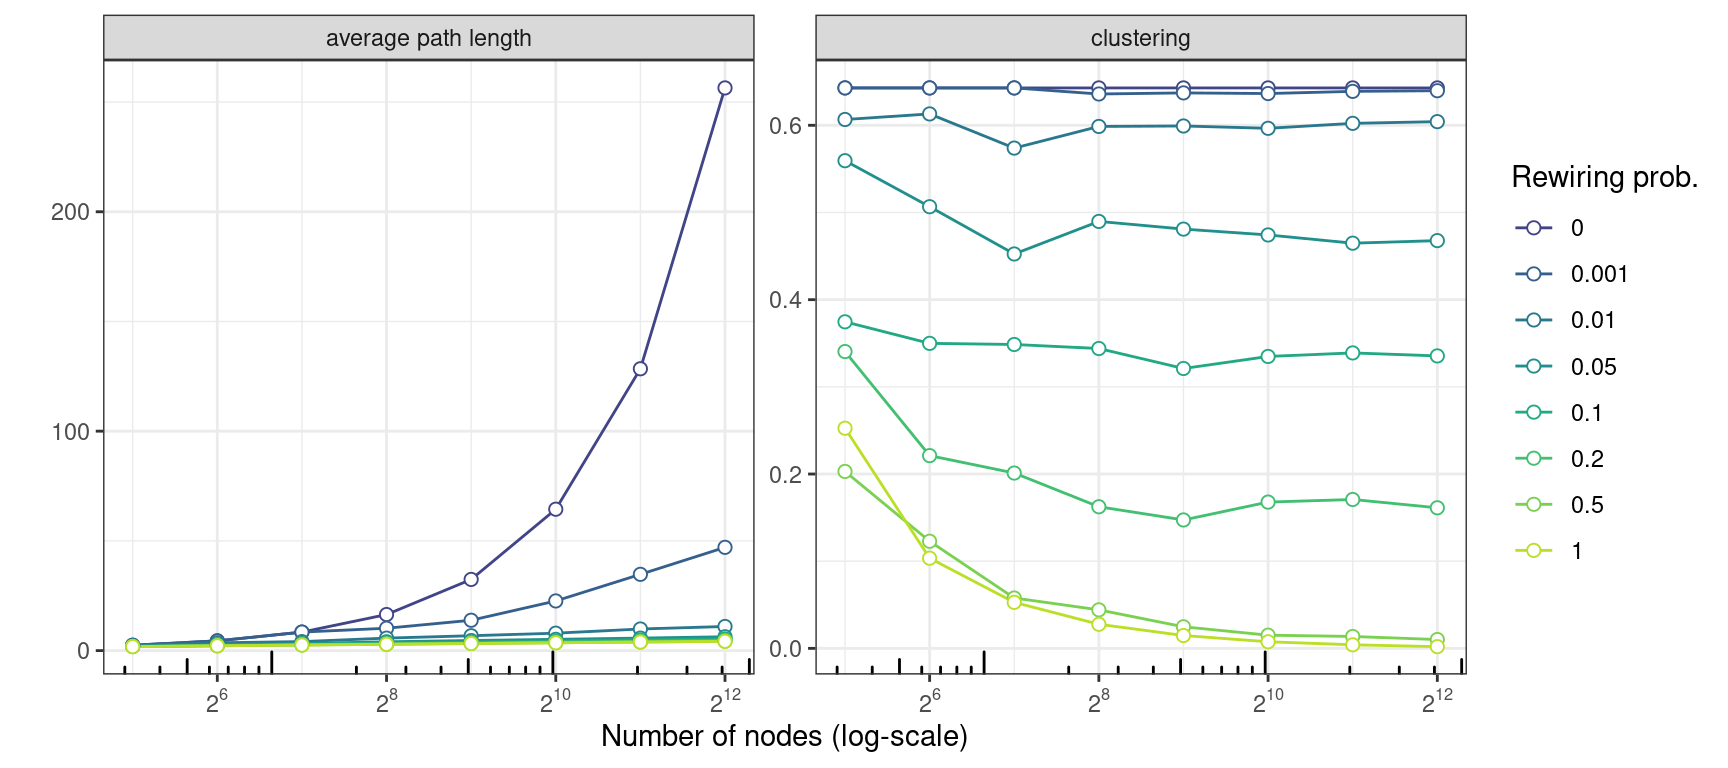
\includegraphics[width=\textwidth]{structure/small_world_simulation_plot-1}
\end{frame}

\section{Assortativity \& homophily}

\begin{frame}{Homophily}
\begin{itemize}
    \item<1-> An important process studied in sociology is \textbf{homophily}.
    \item<2-> In general it refers to a tendency to connect to other people
    who are similar to us (in some important respects).
    \item<3-> It is an important social process as it is one of the main
    drivers of homogenization of social networks (for better or worse).
\end{itemize}
\end{frame}

\begin{frame}{Assortativity}
\begin{itemize}
    \item<2-> In network parlance the tendency of nodes which are similar
    with respect to an attribute is known as \textbf{assortativity}.
    \item<3-> Assortativity can be defined for both qualitative attributes
    (e.g. ethnicity) and numeric features (e.g. age).
    \item<4-> Without going into details, assortativity coefficients are always
    defined as correlations.
    \item<5-> They range from $-1$ (perfect disassortativity) to $1$
    (perfect assortativity).
\end{itemize}
\end{frame}

\begin{frame}{Assortativity of political blogs in the US (2004)}
\centering
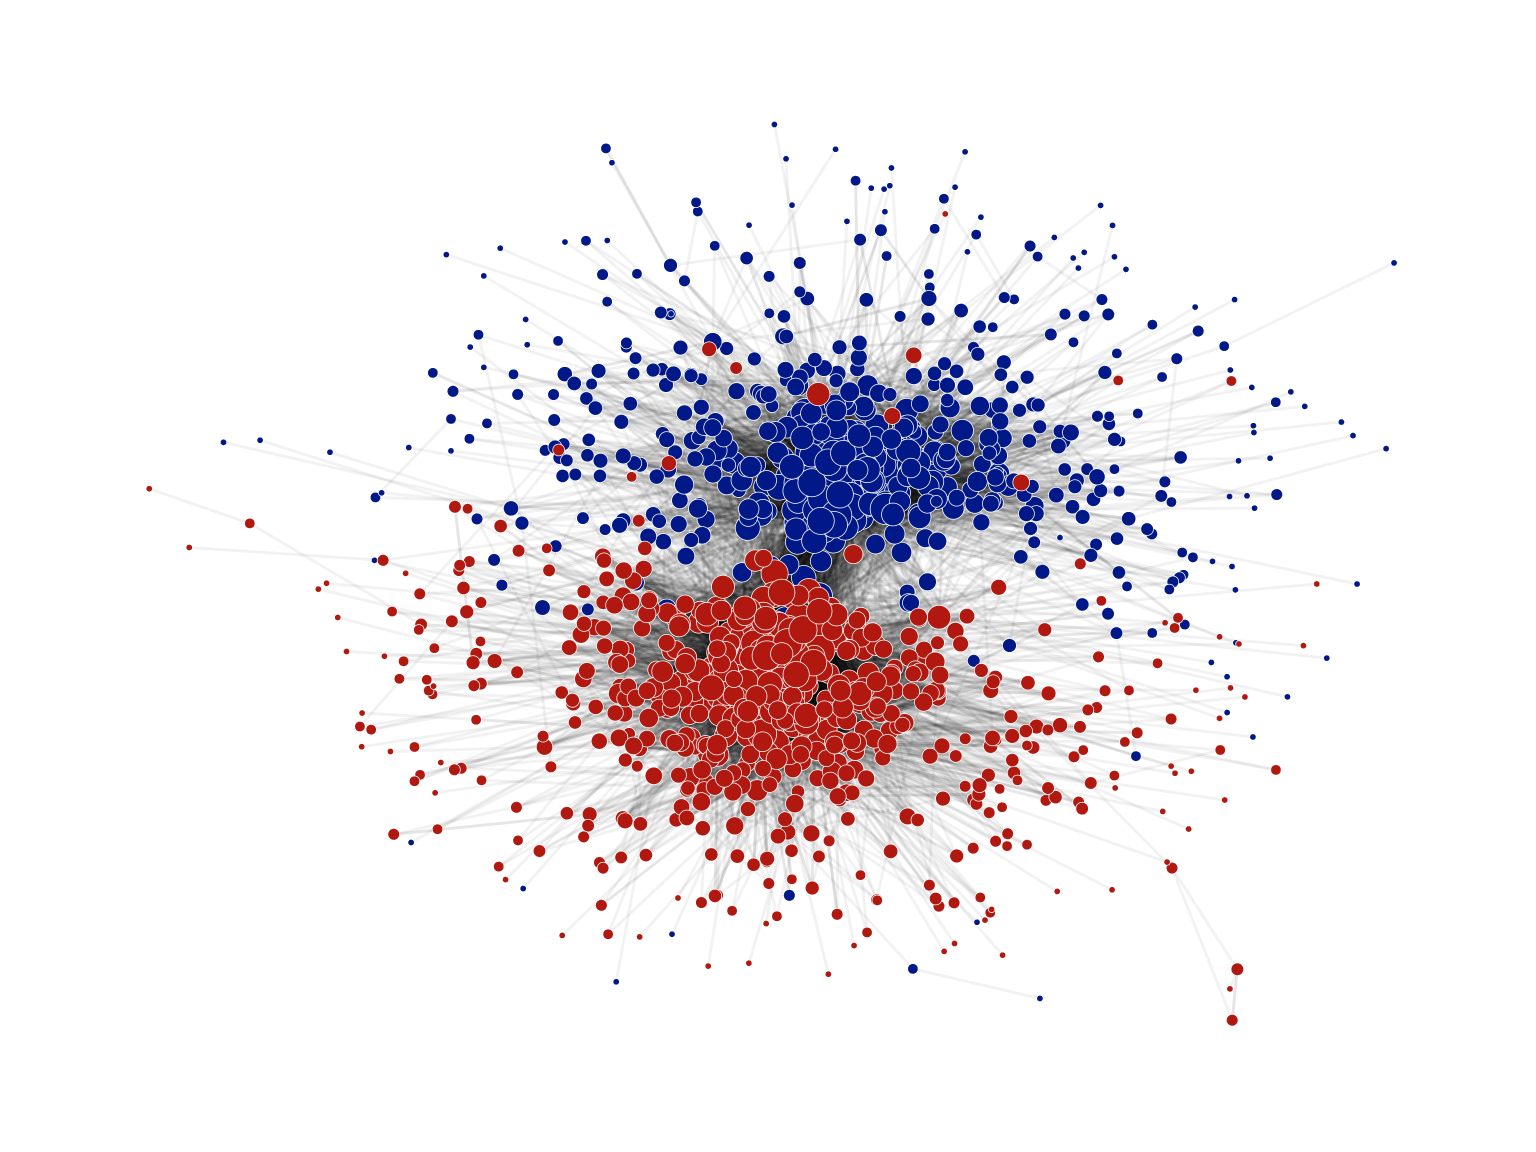
\includegraphics[width=.75\textwidth]{overview/polblogs-1}
\pause
\begin{itemize}
    \item Assortativity with respect to political affiliation
    (democrat vs republican) in this network is very high (about $0.82$).

\end{itemize}
\end{frame}

\section{Structure of social networks}

\begin{frame}{Characteristic structural features of social networks}
\begin{itemize}
    \item It is important that we take a step back now and think about
    characteristic features of social networks.
    \begin{enumerate}
        \item<2-> Right-skewed degree distributions.
        \item<3-> Short average path lengths.
        \item<4-> Non-trivial clustering.
    \end{enumerate}
    \item<5-> The take home message is that any good model of social networks
    should be able to reproduce at least these three properties.
\end{itemize}
\end{frame}

\begin{frame}{Non-trivial clustering}
\begin{itemize}
    \item But what does \textbf{non-trivial clustering} really means?
    \item<2-> In order to answer this question let us first assume that
    social networks are \textbf{sparse}.
\end{itemize}
\end{frame}

\begin{frame}{Sparse networks}
\begin{itemize}
    \item So what are sparse networks then?
    \item<2-> Informally, a sparse network is a network in which only a small
    fraction of all possible edges exist.
\end{itemize}
\end{frame}

\begin{frame}{Sparse network | formalized example}
\begin{itemize}
    \item<2-> Say we have an undirected network in which average node degree,
    $\bar{d}$, is constant irrespective of the number of nodes in the network.
    \item<3-> We have already established that the maximum possible number
    edges in an undirected is:
    \[
        \frac{N(N-1)}{2}
    \]
    \item<4-> And the observed number of edges is just equal to the sum of
    node degrees divided by two:
    \[
        E = \frac{\sum_i d_i}{2} = \frac{N\bar{d}}{2}
    \]
\end{itemize}
\end{frame}

\begin{frame}{Sparse network | formalized example}
    \begin{itemize}
    \item<2-> So the edge density is:
    \[
        \frac{E}{N(N-1)/2} = \frac{N\bar{d}}{N(N-1)}
    \]
    \item<3-> Which in the limit of large $N$ gives:
    \[
        \lim_{N \to \infty} \frac{N\bar{d}}{N(N-1)}
        =
        \lim_{N \to \infty} \frac{\bar{d}}{N-1}
        =
        0
    \]
    \item<4-> In other words, in large sparse networks edge density
    is arbitrarily close to $0$.
\end{itemize}
\end{frame}

\begin{frame}{Clustering in sparse networks is non-trivial}
\begin{itemize}
    \item<2-> Now note that we already established that in the ER model
    expected clustering is equal to $p$, that is, edge density!
    \item<3-> So in sparse random networks clustering is also expected
    to converge to $0$.
    \item<4-> But most social networks are sparse but have non-trivial
    (often very high) clustering.
    \item<5-> And this, arguably, one of the most important properties
    of social networks.
\end{itemize}
\end{frame}

\begin{frame}{Why social networks are sparse?}
\begin{itemize}
    \item<2-> The obvious answer is that \textbf{it depends}.
    \item<3-> But there is also one very important reason, which plays
    a crucial role in particular in the context of friendship and acquaintance
    networks.
\end{itemize}
\end{frame}

\begin{frame}{Dunbar's numbers}
\begin{itemize}
    \item<2-> In short, human beings (and animals too) cannot maintain
    arbitrarily large numbers of contacts.
    \item<3-> Each social tie, depending on its closeness and intensity,
    requires some amount of resources and time involvement.
    \item<4-> Hence, on average there is an upper bound for how many
    social ties we can have.
    \item<5-> And in network terms it means that the average node degree
    in social networks is bounded from above (cannot grow too large).
    \item<6-> So social networks are sparse. \textbf{(QED)}
\end{itemize}
\end{frame}

\begin{frame}{Dunbar's numbers}
\centering
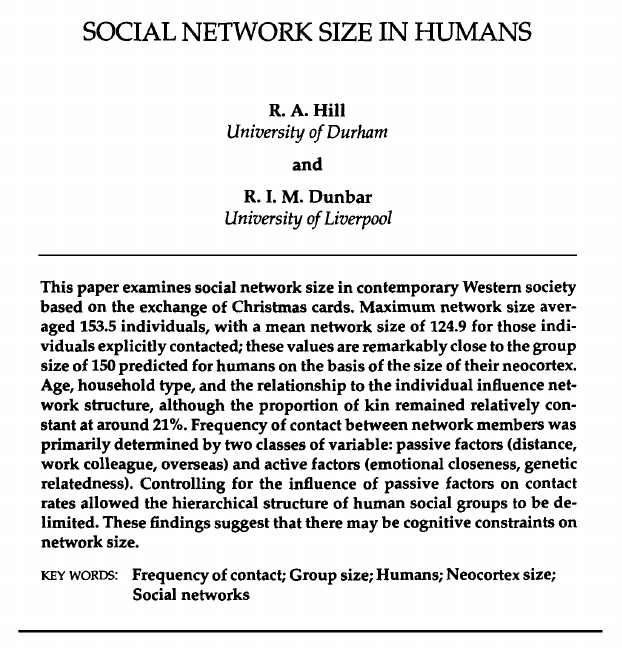
\includegraphics[width=.7\textwidth]{dunbar-numbers}
\end{frame}


\section{Configuration model \& statistical inference}

\begin{frame}{Configration model}
\begin{itemize}
    \item<1-> As we discussed, ER random graph model is usually a poor
    choice for representing generating mechanisms of real networks
    because it cannot produce right-skewed degree distributions.
    \item<2-> So we need a random graph model that would be, well, as random
    as possible except for being able to generate any arbitrary degree
    sequence.
    \item<3-> This is exactly what \textbf{configuration model} does.
\end{itemize}
\end{frame}

\begin{frame}{Configuration model | Outline of the algorithm}
\begin{enumerate}
    \item<1-> Take an arbitrary degree sequence (for instance a sequence of node
    degrees from an observed network of interest).
    \item<2-> Initialize a network with $N$ nodes and no edges.
    \item<3-> To each node assign a number of \textbf{stubs} or
    \textbf{half-links} equal to its desired degree.
    \item<4-> Sample two nodes with at least one open stub uniformly at random,
    connect them and decrease the numbers of their stubs by $1$.
    \item<5-> Repeat (4) until there are no more nodes with open stubs.
\end{enumerate}
\end{frame}

\begin{frame}{Configuration model | Example}
\begin{center}
\begin{tikzpicture}[node distance=1cm]
    % Nodes
    \node[vertex] (n1) {$1$};
    \node[above left of=n1] (n1s1) {};
    \node[above right of=n1] (n1s2) {};
    \node[above left of=n1s1] (n2s1) {};
    \node[above right of=n1s2] (n3s1) {};
    \node[vertex, above left of=n2s1] (n2) {$2$};
    \node[vertex, above right of=n3s1] (n3) {$3$};
    % Edges
    \path[draw, ultra thick]
    (n1) -- (n1s1)
    (n1) -- (n1s2)
    (n2) -- (n2s1)
    (n3) -- (n3s1);
    \pause
    \path[draw, ultra thick]
    (n2) -- (n1);
    \pause
    \path[draw, ultra thick]
    (n3) -- (n1);
\end{tikzpicture}
\end{center}
\end{frame}

\begin{frame}{Configuration model | Some remarks}
\begin{itemize}
    \item<2-> There are of course a lot of technicalities involved
    in this process which we conveniently omitted.
    \item<3-> However, the point is that configuration model gives us
    a null model which is surprisingly useful in many situations.
    \item<4-> In particular, it can be used to define proper statistical tests
    for determining whether a given structural property of a network
    is indicative of some non-trivial generating mechanisms or can be
    attributed simply to the effect induced by the degree sequence of the
    network alone.
\end{itemize}
\end{frame}

\begin{frame}{Statistical tests based on configuration model}
\begin{enumerate}
    \item<2-> Generate $K$ randomized networks based on configuration model
    with the the same degree sequence as in an observed network of interest.
    \item<3-> Calculate any statistic of interest for each of the $K$ networks.
    The whole set of calculated values is an approximation to the
    \textbf{null distribution} of the statistic under the configuration model.
    \item<4-> Compare an observed value of the statistic to the null distribution.
    \item<5-> In particular, one can calculate the fraction of null distribution
    which is greater than or equal to the observed value. This gives a proper
    $p$-value (statistical significance) for the observed statistic
    (relative to the null model).
\end{enumerate}
\end{frame}

\begin{frame}{Statistical test for clustering | Example}
\centering
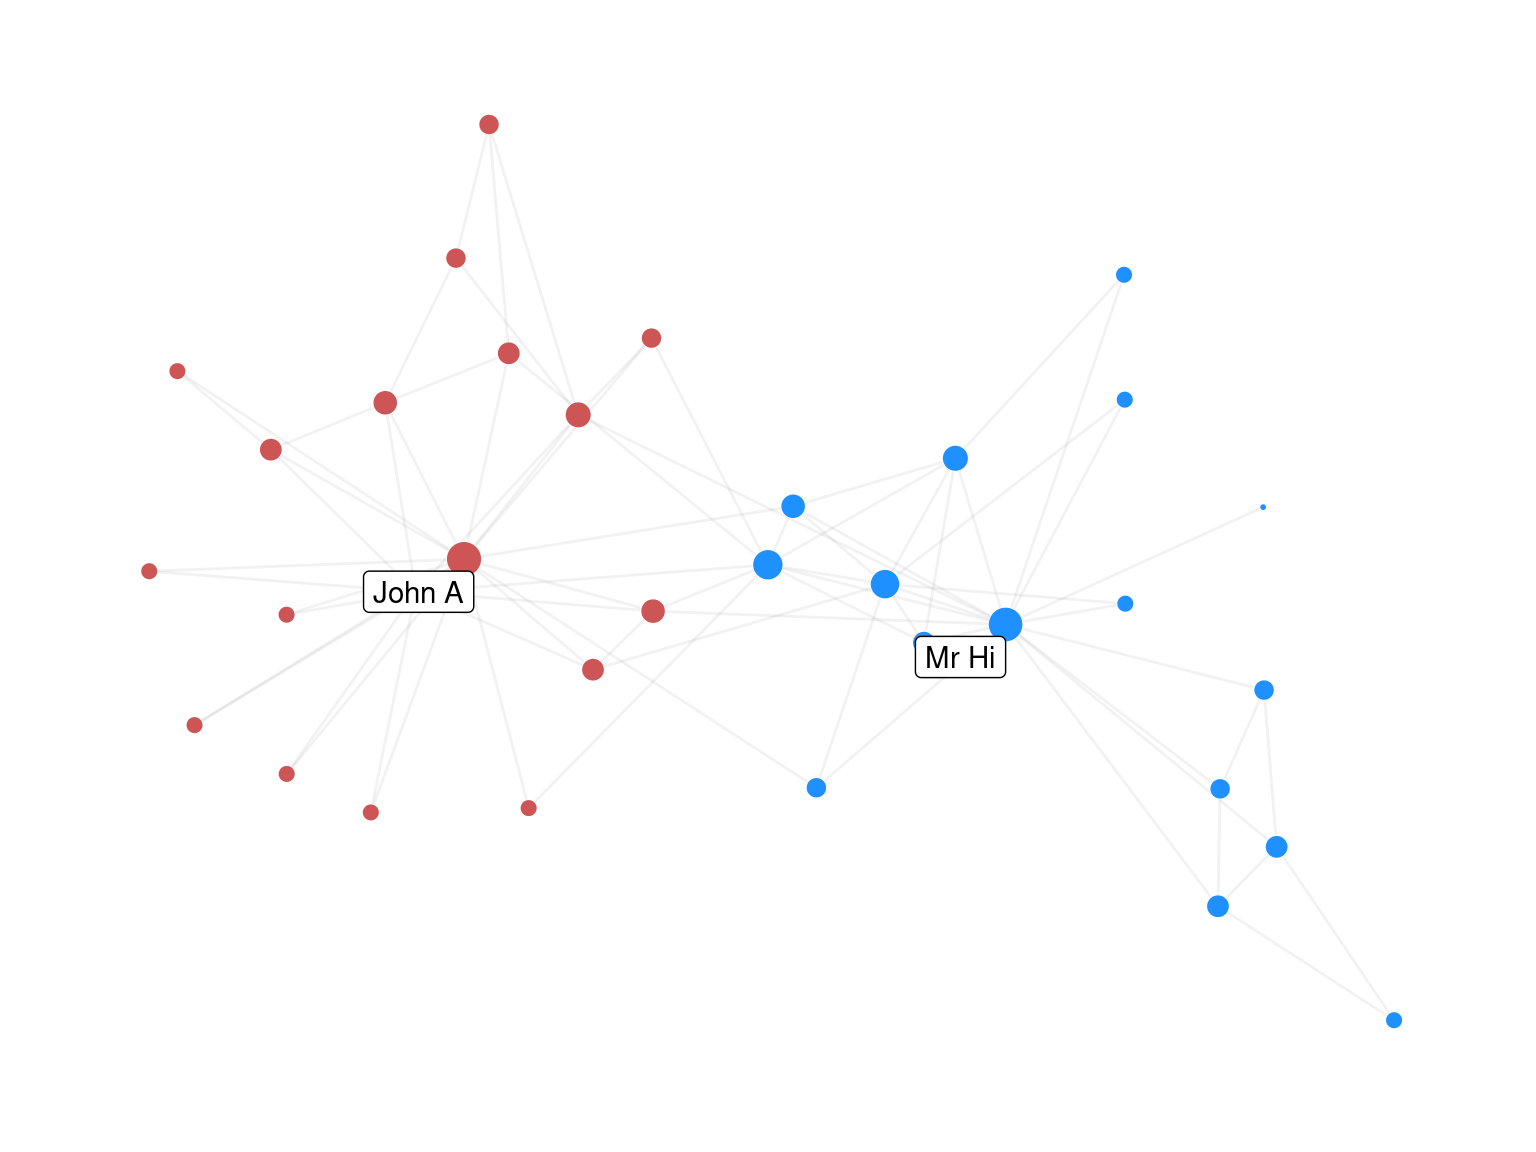
\includegraphics[width=.9\textwidth]{overview/karate-1}
\end{frame}

\begin{frame}{Statistical test for clustering | Example}
\begin{itemize}
    \item<2-> In the Zachary's Karate Club network observed global
    clustering is about $0.255$ and edge density about $0.139$.
    \item<3-> This indicates that clustering is not trivial with
    respect to the ER model.
    \item<4-> But what happens if take the degree sequence for granted?
\end{itemize}
\end{frame}

\begin{frame}{Statistical test for clustering | Example}
\centering
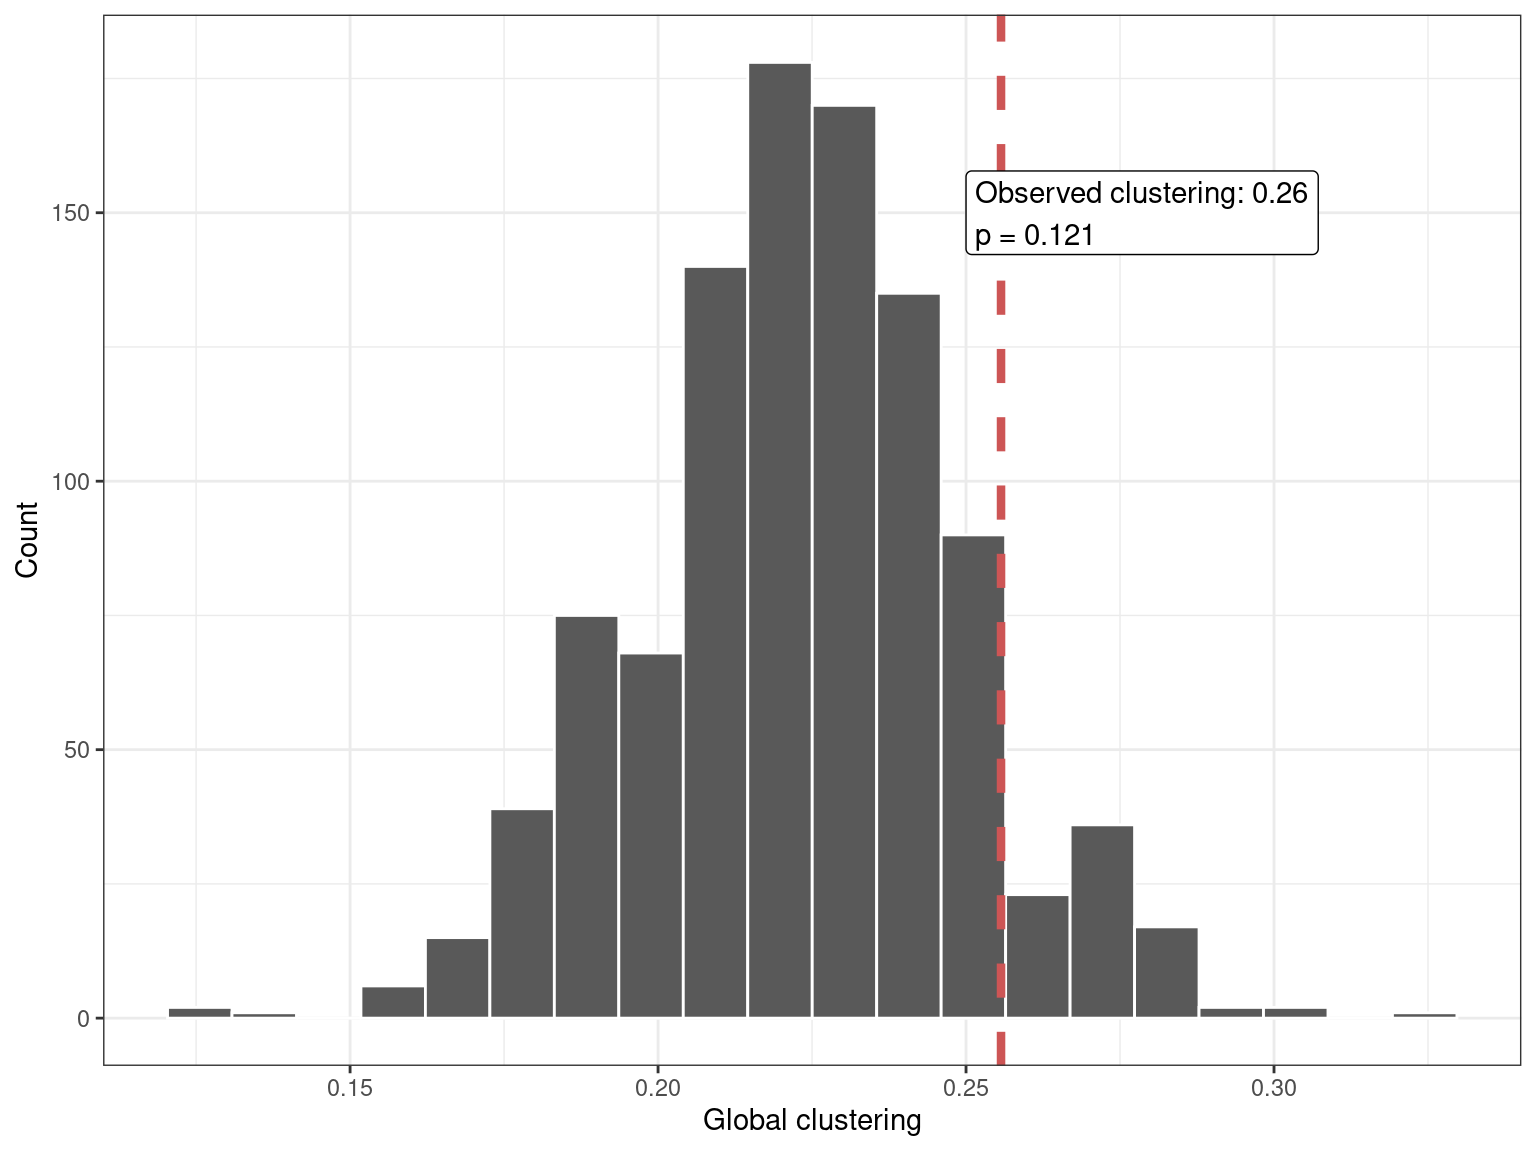
\includegraphics[width=.9\textwidth]{structure/conf_model_karate_plot-1}
\end{frame}

{%<--- Start local changes
\setbeamertemplate{navigation symbols}{}
\usebackgroundtemplate{
    \hspace{-1em}
    
\includegraphics[width=1.03\paperwidth]{thats-all-folks}
}
\begin{frame}{Thank you! Questions?}
\hfill
\begin{minipage}{.65\textwidth}
    \vspace{14.4em}
    \begin{tcolorbox}[
        width=1.1\textwidth,
        colback=black!5,
        title=\textbf{Contact}
    ]
    \texttt{\scriptsize{
        \hspace{-1.2em}
        \faIcon{envelope}\enspace
        \textcolor{blue}{\href{mailto:stalaga@uw.edu.pl}{stalaga@uw.edu.pl}} \\
        \faIcon{address-card}
        \href{http://iss.uw.edu.pl/en/szymon-talaga/}{iss.uw.edu.pl/en/szymon-talaga}
    }}
    \end{tcolorbox}
\end{minipage}
\end{frame}
}%<---- Finish local changes


\section{More on networks}

\begin{frame}{Textbook by Wasserman \& Faust}
\centering
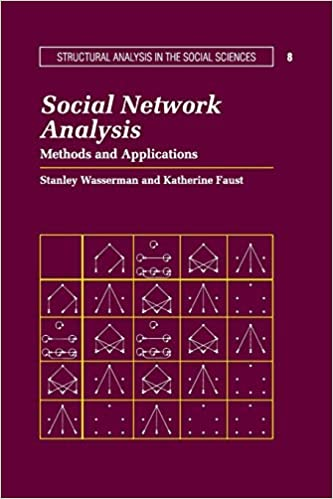
\includegraphics[width=.25\textwidth]{wasserman-faust}
\blfootnote{%
    A classic textbook on social networks analysis for social scientists.
    It is a little outdated but gives a great overview of main methods
    and the history of the field. Moreover, it is not very math-heavy,
    so is a good choice for people starting with network science, who
    do not have a solid technical background.
}
\end{frame}

\begin{frame}{Textbook by Newman}
\centering
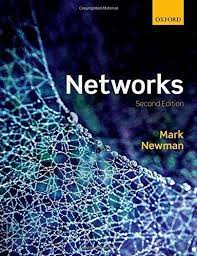
\includegraphics[width=.25\textwidth]{newman-book}
\blfootnote{%
    A modern classic giving a great overview of network science including
    perspectives of multiple fields from physics and computer science to
    biology and sociology. It is, however, more math-heavy so some background
    in general math, probability theory, statsitics, linear algerba etc.
    is recommended.
}
\end{frame}

\begin{frame}{Geometric take on structure of social networks}
\centering
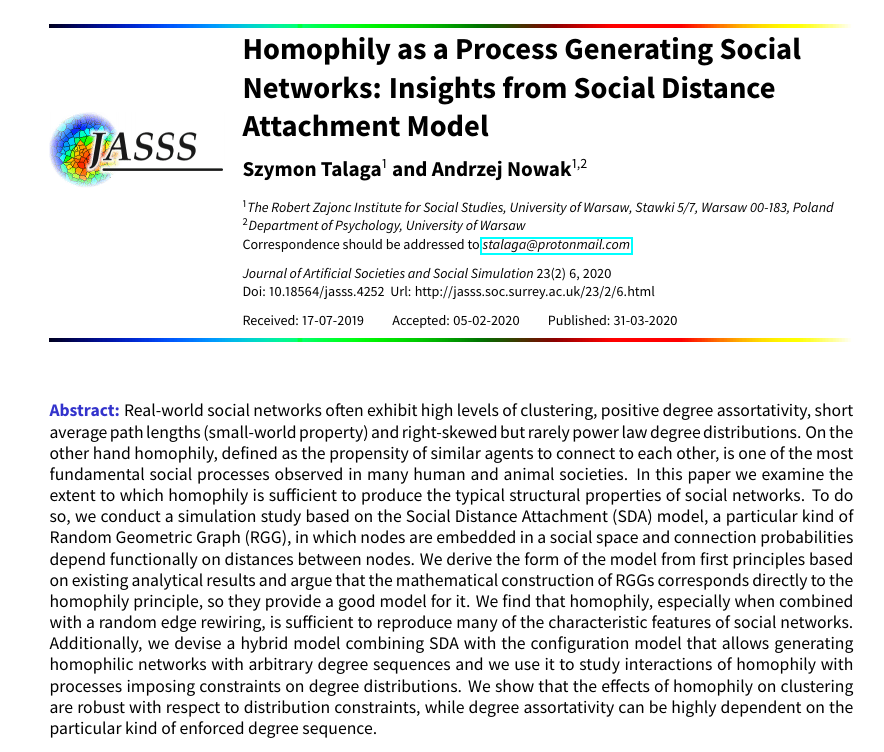
\includegraphics[width=.5\textwidth]{jasss}
\blfootnote{%
    A quite extensive discussion of characterisitc features of social networks
    and possible generating mechanisms from the vantage point of homophily
    and geometric network models (for which, alas, we did not have time!)
    by Yours Truly. It touches a lot of topics that we briefly mentioned
    in this presentation such as sparsity and Dunbar's numbers or configuration
    models. It also contains a lot of useful references.
}
\end{frame}

\begin{frame}{The House of Medici rise to power in medieval Florence}
\centering
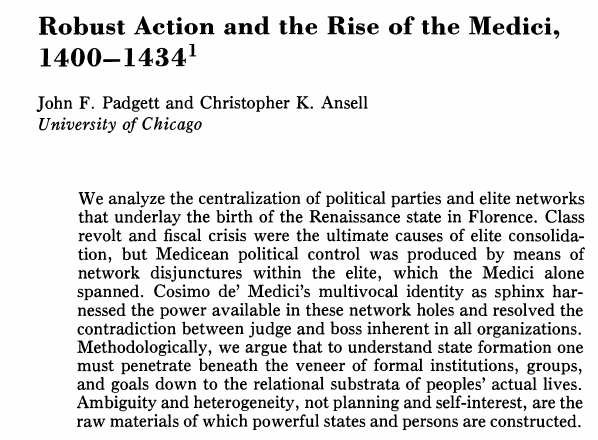
\includegraphics[width=.6\textwidth]{padgett}
\blfootnote{%
    In mu humble opinion, one of the greatest sociological papers ever,
    which is also concerned with the topic of political struggles and elites.
    It explores, via network methods, a historical trajectory and strategy
    that allowed Medici to take control over medieval Florence.
}
\end{frame}

\end{document}
